%
% main.tex -- Paper zum Thema visuell
%
% (c) 2019 Hochschule Rapperswil
%
\chapter{Gabor-Wavelets und visuelle Wahrnehmung\label{chapter:visuell}}
\lhead{Gabor-Wavelets und visuelle Wahrnehmung}
\begin{refsection}
\chapterauthor{Raphael Unterer}

\section{Einleitung}
\rhead{Einleitung}

Die visuelle Wahrnehmung des Menschen ist spezialisiert auf das erkennen von Mustern und Objekten.
Bilder vom menschlichen Auge werden im Visuellen Kortex 1 vorverarbeitet.
Diese Vorverarbeitung kann mit Hilfe von 2-dimensionalen Gabor-Wavelets modelliert werden.

Viele Probleme im Bereich des maschinellen Lernens versuchen ebenfalls Objekte auf Bildern zu erkennen.
Vor allem Convolutional Neural Networks (CNN) zeigen gute Ergebnisse.
Dementsprechend wäre es interessant zu Wissen ob eine Vorverarbeitung mit Hilfe von Gabor-Wavelets eine Verbesserung der CNNs erreicht werden kann.

Das Ziel dieses Papers ist es, alle diese Dinge (Gabor-Wavelets, Neurologie und CNNs) genauer zu analysieren.
Abschliessend wird in einem Experiment gezeigt ob eine Gabor-Wavelet-Transformation als Vorverarbeitung Sinn macht.



\section{Zweidimensionales Gabor-Wavelet}
\rhead{Zweidimensionales Gabor-Wavelet}

Die Idee des eindimensionalen Gabor-Wavelets wird zuerst als Grundlage genommen. 
Daraus wird dann das zweidimensionale Wavelet abgeleitet und die entstehenden Freiheitsgrade erläutert.

\subsection{Gabor-Wavelet}

Bei der Wavelet-Transformation besteht eine Zeit-Frequenz-Unschärfe.
Diese Unschärfe bewirkt, dass die Auflösung im Zeitbereich umgekehrt proportional zur Auflösung im Frequenzbereich ist.
Das Gabor-Wavelet stellt einen optimalen Kompromiss aus Zeit-und Frequenzauflösung dar.
Die Anwendung des Wavelets minimiert dabei das Produkt der Standardabweichungen im Zeit- und Frequenzbereich. \cite{paper:communication}
%TODO more details?

Ein solches Gabor-Wavelet besteht aus einer komplexen Schwingung, welche mit einer Gaussfunktion gefenstert ist und somit exponentiell abfällt.

\begin{equation}
G(x)= e^{-\frac{(x-x_{0})^{2}}{\sigma^{2}}} e^{i\xi_{0}x}
\end{equation}

Der Parameter $\sigma$ beschreibt die Standardabweichung der Gaussfunktion und $\xi$ die Frequenz der komplexen Schwingung. 
Die komplexe Schwingung besteht aus einem Sinus und einem  Kosinus Anteil. 
Ein Beispiel eines Sinus-Gabor-Wavelet wird in Abbildung \ref{fig:gabor1d} gezeigt.

\begin{figure}
	\centering
	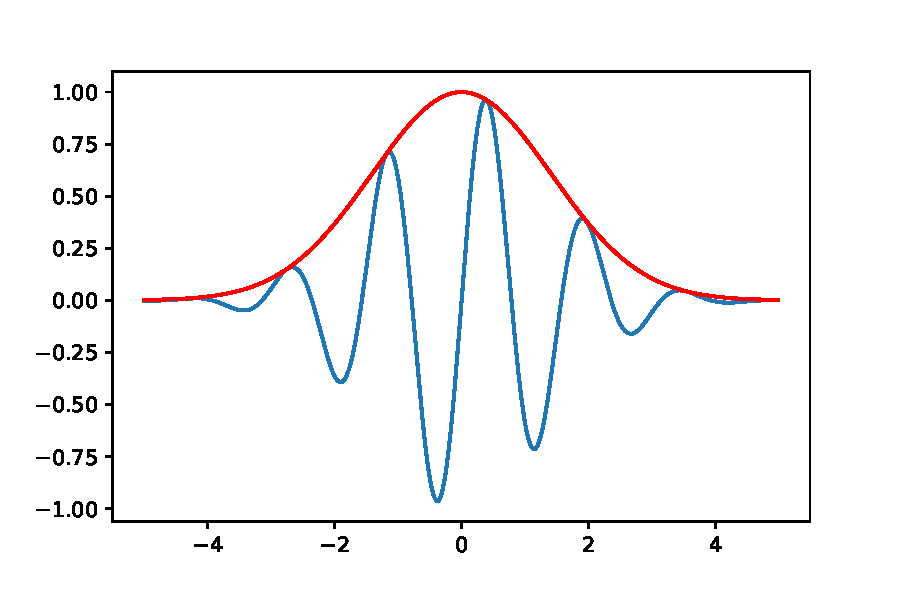
\includegraphics[width=0.7\linewidth]{./papers/visuell/images/gabor_1d}
	\caption{Beispiel eines Sinus-Gabor-Wavelets}
	\label{fig:gabor1d}
\end{figure}


\subsection{Erweiterung auf zwei Dimensionen}

Um ein solches Wavelet auf ein Bild anwenden zu können, ist es sinnvoll dieses auf zwei Dimensionen zu erweitern.
Diese Erweiterung ergibt die folgende Formel:

\begin{equation}
G(x,y)= e^{-(\frac{(x-x_{0})^{2}}{\sigma^{2}}+\frac{(y-y_{0})^{2}}{\beta^{2}})}
e^{i(\xi_{0}x+\nu_{0}y)}.
\end{equation}

Das zweidimensionale Wavelet besteht immer noch aus einer komplexen Schwingung multipliziert mit einer elliptischen Gaussfunktion. 
Diese Schwingung kann man sich als ebene Welle vorstellen, welche abhängig von $\xi$ und $\nu$ in eine bestimmte Richtung zeigt (vgl. Abbildung \ref{fig:planarwave}).

\begin{figure}
	\centering
	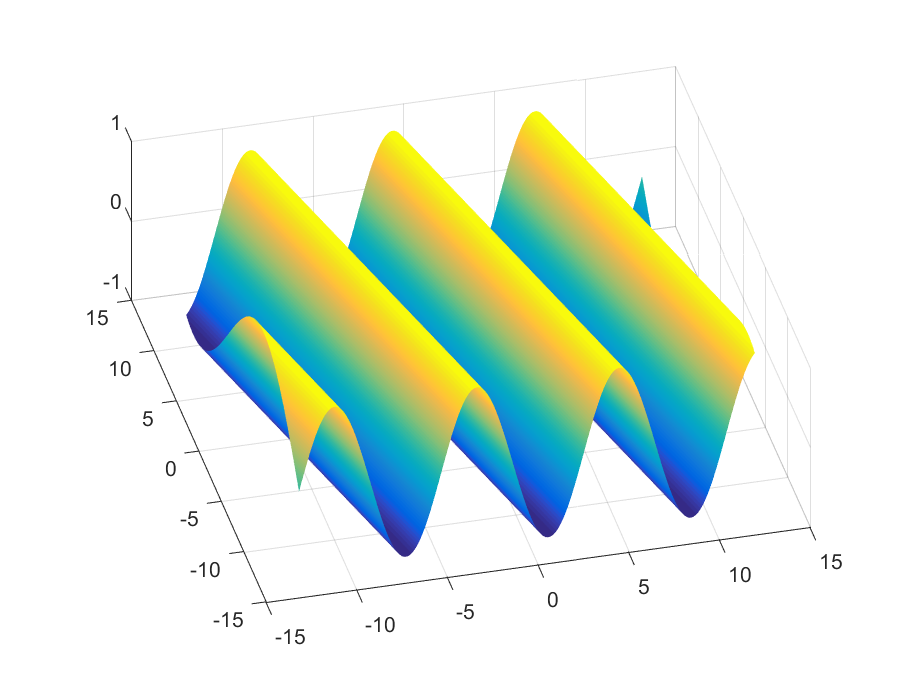
\includegraphics[width=0.7\linewidth]{./papers/visuell/images/planarwave.eps}
	\caption{Beispiel einer ebenen Welle}
	\label{fig:planarwave}
\end{figure}



Diese Parameter ($\sigma$, $\beta$, $\xi$, $\nu$) dieser Formel sind unhandlich und es ist nicht offensichtlich was eine Änderung dieser bewirkt.
Also ersetzen wir diese durch neue Parameter und erhalten 

\begin{equation}
G(x,y)=e^{-\frac{x'^{2}+\gamma^{2}y'^{2}}{2\sigma^{2}}}
e^{i(2\pi\frac{x'}{\lambda} + \phi)},
\end{equation} 
wobei $x'=x\cos(\theta)+y\sin(\theta)$ und $y'=-x\sin(\theta)+y\cos(\theta)$.
Der Parameter $\gamma$ beschreibt das Verhältnis der Streckung in $x$- und $y$-Richtung.
Diese Streckung der elliptischen Gaussfunktion bestimmt ob das Wavelet eher rund oder länglich ist.
Die Standardabweichung der Gausskurve welche mit der Schwingung multipliziert wird ist als Parameter $\sigma$ definiert.
Grösseres $\sigma$ bewirkt ein breiteres Wavelet.
Die komplexe Schwingung wird durch die Wellenlänge $\lambda$ und die Phase $\phi$ definiert.
Der Parameter $\theta$ definiert nun die Ausrichtung der komplexen Schwingung.
Eine Änderung von $\theta$  bewirkt somit eine Drehung der Wellenfronten.
Der letzte Parameter $\phi$ bewirkt eine Phasenverschiebung der Schwingung. 
Da eine solche Phasenverschiebung keinen klaren Nutzen zu haben scheint, wird $\phi=0$ gesetzt.

Wie sich Gabor-Wavelets in Abhängigkeit dieser Parameter Verhalten zeigt Abbildung \ref{fig:kernels}.
Vier unabhängige Freiheitsgrade (Parameter) sind zu viel um als Mensch einen guten Überblick zu behalten.
Aus diesem Grund werden im weiteren Verlauf dieses Papers die Gausskurven-Parameter $\sigma$ und $\gamma$ fixiert und nur noch die anderen beiden Parameter verändert.

\begin{figure}
	\centering
	\subfigure[Parameter der Gaussfunktion $\gamma$ und $\sigma$ werden verändert]{\label{fig:kernels_a}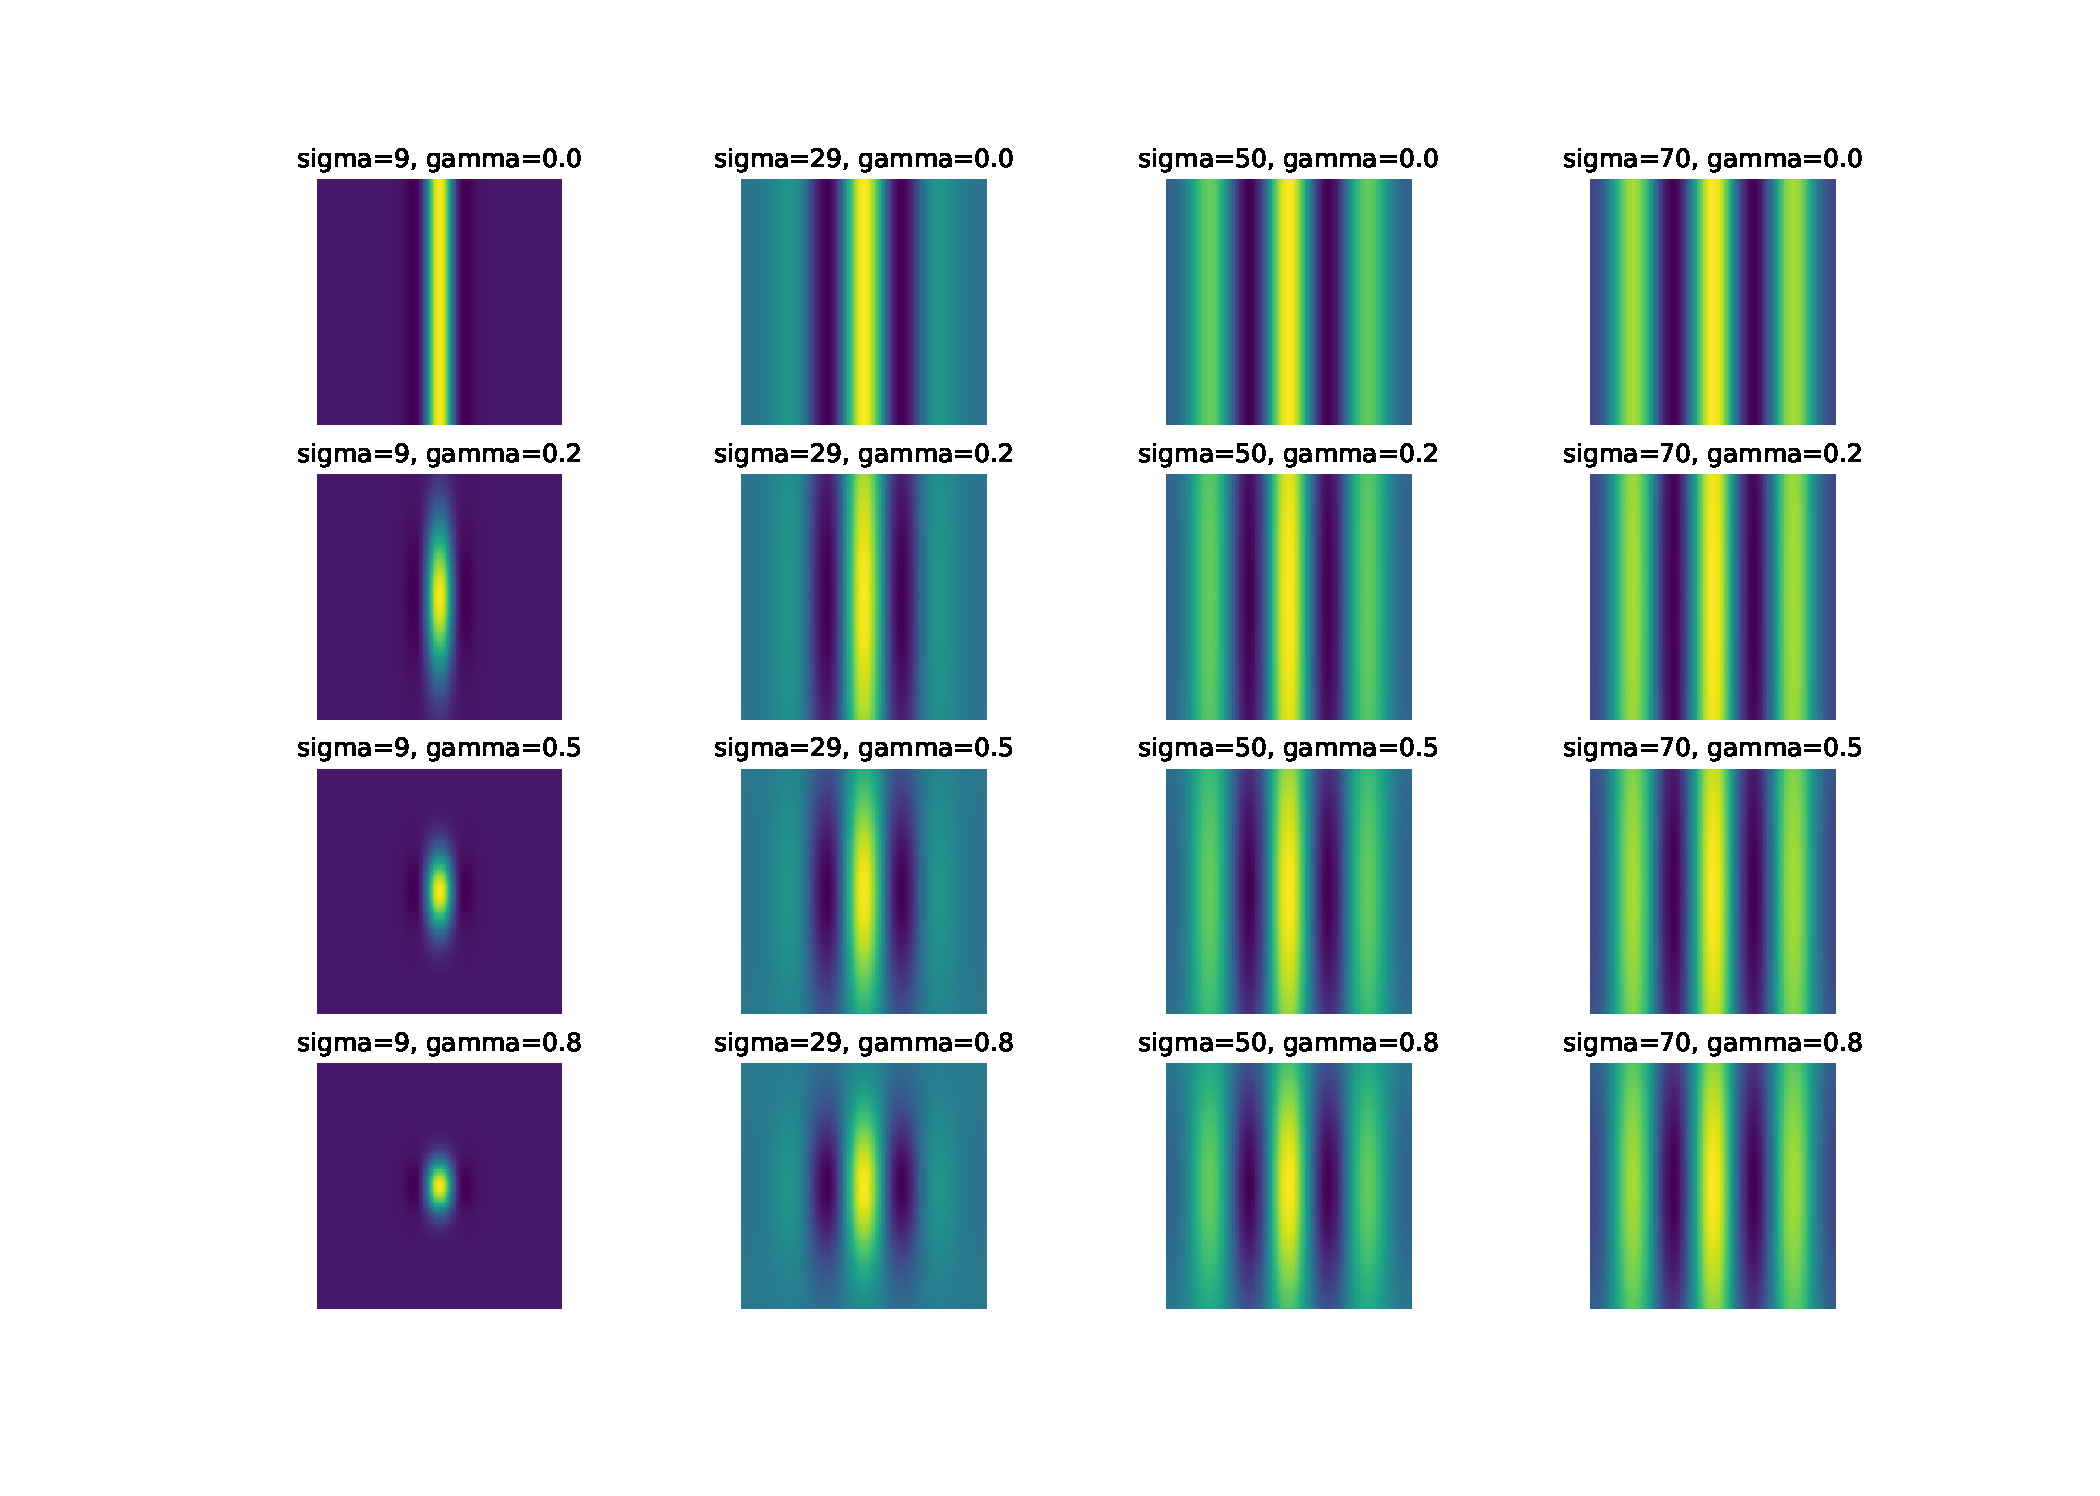
\includegraphics[width=0.45\linewidth]{./papers/visuell/images/kernels_sigma_gamma.pdf}}
	
	\subfigure[Wellenlänge der Schwingung $\lambda$ und Ausrichtung $\theta$ werden verändert]{\label{fig:kernels_b}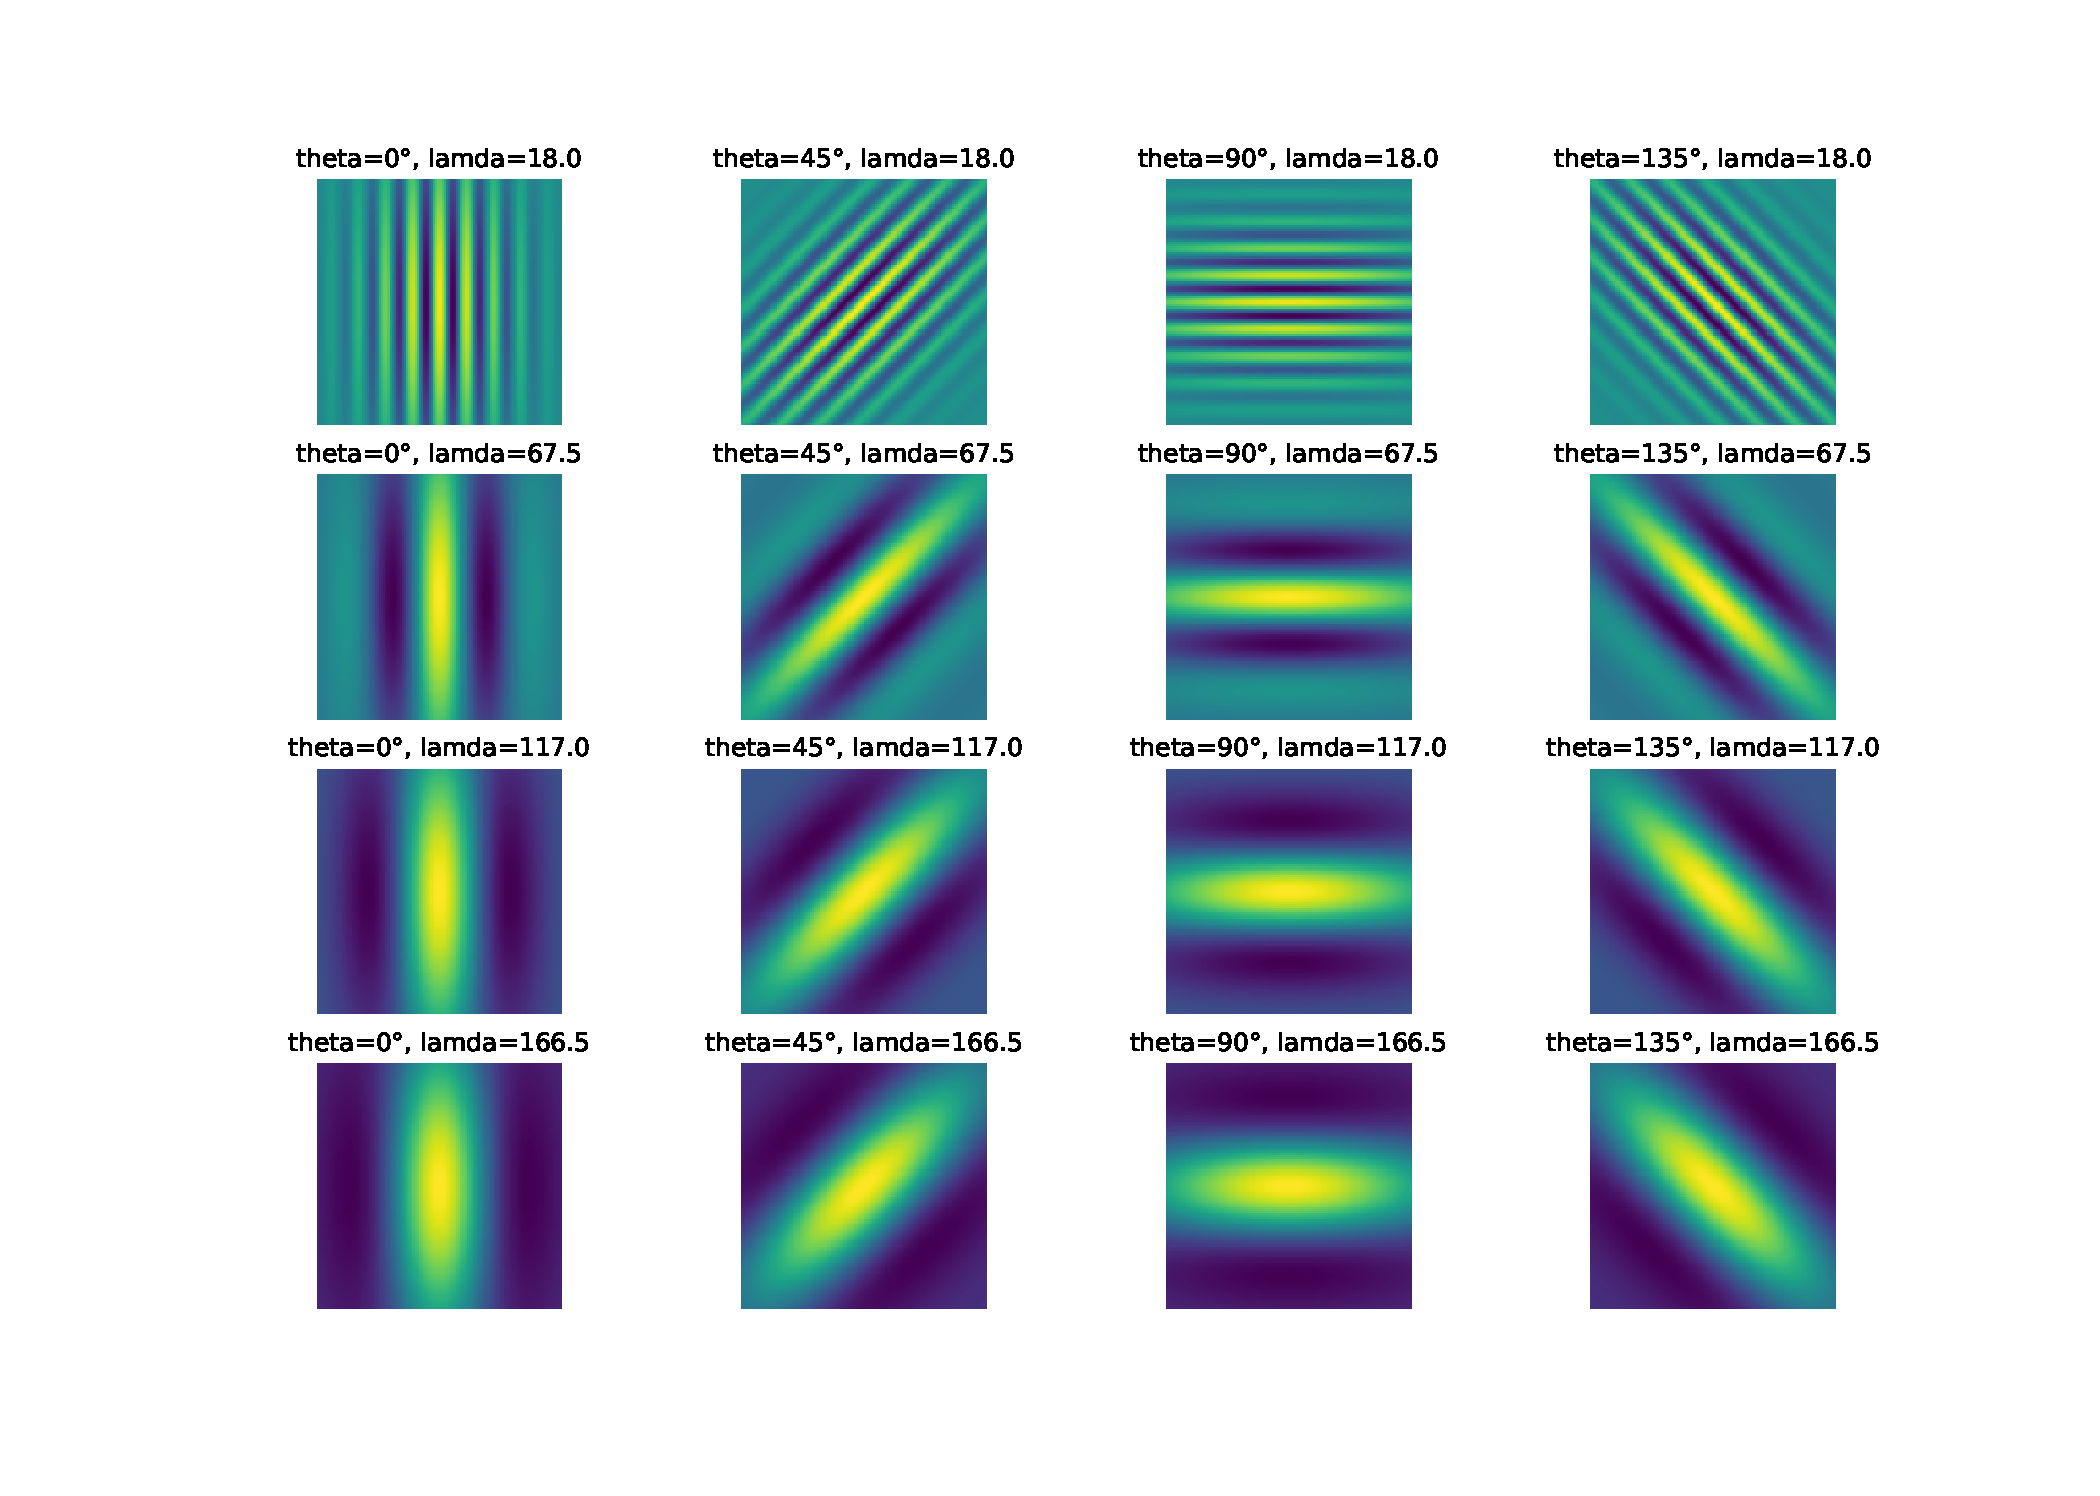
\includegraphics[width=0.45\linewidth]{./papers/visuell/images/kernels_theta_lambda.pdf}}
	\caption{Abhängigkeit des Gabor-Wavelets von den Parametern}
	\label{fig:kernels}
\end{figure}

\section{Visuelle Wahrnehmung}
\rhead{Visuelle Wahrnehmung}

In den vorherigen Abschnitten haben wir das zweidimensionale Gabor-Wavelet genauer betrachtet.
Dieses Wavelet ist einerseits der optimale Kompromiss zwischen Zeit- und Frequenzauflösung und andererseits kann es in verschiedene Richtungen ausgerichtet werden.
Diese speziellen Eigenschaften sind sehr nützlich und es zeigte sich, dass die Hirne von Säugetieren ähnliche Eigenschaften besitzen.
In den folgenden Abschnitten wird versucht zu zeigen, was die visuelle Wahrnehmung und Gabor-Wavelets gemeinsam haben. 

\subsection{Primärer Visueller Kortex}\label{subsec:v1}

Der primäre Visuelle Kortex (V1) verarbeitet die Bildinformationen welche vom Auge aufgenommen werden.
Als Ausgangsprodukt stellt er abstrakte Features zu Verfügung, welche dann vom Hirn zusammen mit weiteren Informationen (Kontextwissen, andere Sinne)  benützt werden, um Objekte zu erkennen.
Erste Analysen des V1 wurden von Hubel und Wiesel bereits 1959 veröffentlicht \cite{paper:hubelwiesel}.
Ihre Erkenntnisse haben sie anhand von Versuchen an Katzenhirnen gewonnen.

Jedes Neuron innerhalb des V1 bekommt Eingangssignale einer bestimmten Region der Netzhaut.
Eine solche Region wird rezeptives Feld genannt.
Diese rezeptiven Felder bestimmen also welcher Teil eines Bildes vom Neutron bearbeitet wird.
Es gibt verschiedene Arten von Neuronen innerhalb des V1.
Eine wichtige Gruppe davon sind die sogenannten einfachen Zellen.
Diese zeigen ein orientierungsspezifisches Antwortverhalten auf optische Inputs.
Ausserdem beinhalten die einfachen Zellen immer abwechselnde ON und OFF Regionen, welche ansprechen bei Licht (ON) oder eben keinem Licht (OFF).
Die zweite wichtige Gruppe der Neuronen sind die komplexen Zellen.
Diese können als Kombination von mehreren einfachen Zellen modelliert werden, wobei alle einfachen Zellen in die selbe Richtung orientiert sind.
Allerdings ist diese Erklärung der komplexen Zellen nicht überall anerkannt \cite{book:neuroscience}.


\subsection{Modellierung der Funktion des V1 mithilfe von Gabor-Wavelets}

Die Eigenschaften der einfachen Zellen sind sehr ähnlich derjenigen des Gabor-Wavelets.
Deshalb haben Forscher begonnen die einfachen Zellen mit Hilfe von Gabor-Wavelets zu modellieren \cite{paper:imgrep}.
Analog zu den einfachen Zellen können Gabor-Wavelets ebenfalls in beliebige Richtungen ausgerichtet und deren Wellenlänge variiert werden.
Ausserdem kann die Schwingung des Gabor-Wavelets als ON-OFF-Pattern interpretiert werden.
Dies ist eine sehr schöne Entdeckung, da es zeigt, dass sich der V1 während der Evolution hin zu einem optimalen Kompromiss aus Zeit- und Frequenzinformationen entwickelt hat.
Die Eigenschaften des Gabor-Wavelets sollten auch für die künstliche Bilderkennung sinnvoll sein, da es offensichtlich einen evolutionären Vorteil darstellt wenn Bilder in dieser Art vorverarbeitet werden.
\section{Künstliches Neuronales Netz}
\rhead{Künstliches Neuronales Netz}

Künstliche neuronale Netze (KNN) stellen eine Möglichkeit des maschinellen Lernens dar, welche vom Hirn inspiriert wurde.
Ein KNN besteht aus verschiedenen Neuronen, welche hierarchisch in sogenannten Layern angeordnet werden (vgl. Abbildung \ref{fig:neuralnet}).
Jeder Eingangswert $x_i$ zu einem Neuron wird mit einem Faktor $w_i$ multipliziert.
Alle gewichteten Eingänge werden zusammen mit einem Schwellenwert $b$ addiert.
Diese Summe wird danach durch eine nichtlineare Aktivierungsfunktion $H$ aktiviert und bildet so den Ausgang $y$
\begin{equation} \label{eq:neuron}
y=H\left(\sum_{i} x_i w_i+b\right).
\end{equation}
Die Nichtlinearität ist entscheidend um nichtlineare Probleme lösen zu können.
Der Aufbau eines Neuron ist in Abbildung \ref{fig:neuron} gezeigt. 

\begin{figure}
	\centering
	\def\layersep{2.5cm}

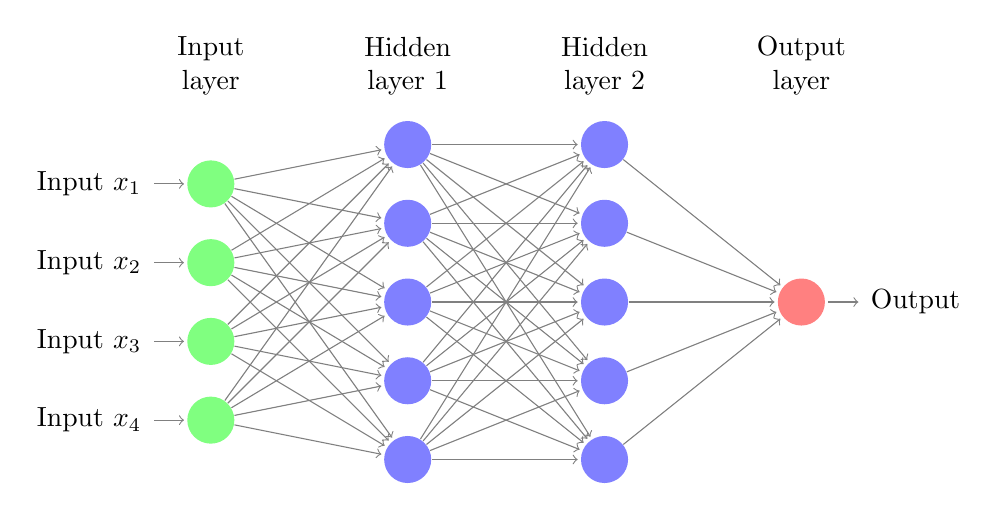
\begin{tikzpicture}[shorten >=1pt,->,draw=black!50, node distance=\layersep]
\tikzstyle{every pin edge}=[<-,shorten <=1pt]
\tikzstyle{neuron}=[circle,fill=black!25,minimum size=17pt,inner sep=0pt]
\tikzstyle{input neuron}=[neuron, fill=green!50];
\tikzstyle{output neuron}=[neuron, fill=red!50];
\tikzstyle{hidden neuron}=[neuron, fill=blue!50];
\tikzstyle{hidden neuron 2}=[neuron, fill=blue!50];
\tikzstyle{annot} = [text width=4em, text centered]

% Draw the input layer nodes
\foreach \name / \y in {1,...,4}
	\node[input neuron, pin=left:Input $x_{\y}$] (I-\name) at (0,-\y) {};

% Draw the hidden layer 1 nodes
\foreach \name / \y in {1,...,5}
	\path[yshift=0.5cm]
		node[hidden neuron] (H-\name) at (\layersep,-\y cm) {};

% Draw the hidden layer 2 nodes
\foreach \name / \y in {1,...,5}
	\path[yshift=0.5cm]
		node[hidden neuron 2] (H2-\name) at (2*\layersep,-\y cm) {};

% Draw the output layer node
\node[output neuron,pin={[pin edge={->}]right:Output}, right of=H2-3] (O) {};

% Connect every node in the input layer with every node in the
% hidden layer.
\foreach \source in {1,...,4}
	\foreach \dest in {1,...,5}
		\path (I-\source) edge (H-\dest);
\foreach \source in {1,...,5}
	\foreach \dest in {1,...,5}
		\path (H-\source) edge (H2-\dest);

% Connect every node in the hidden layer with the output layer
\foreach \source in {1,...,5}
	\path (H2-\source) edge (O);

% Annotate the layers
\node[annot,above of=H-1, node distance=1cm] (hl) {Hidden layer 1};
\node[annot,left of=hl] {Input layer};
\node[annot,right of=hl] (hl2) {Hidden layer 2};
\node[annot,right of=hl2] {Output layer};
\end{tikzpicture}

	\caption{Aufbau eines neuronalen Netzes mit zwei hidden Layern (blau) und einem output Layer (rot). Die blauen und roten Kreise stellen also die Neuronen dar, die Grünen sind der Input.}
	\label{fig:neuralnet}
\end{figure}

\begin{figure}
	\centering
	\tikzstyle{inputNode}=[draw,circle,minimum size=10pt,inner sep=0pt]
\tikzstyle{stateTransition}=[->, thick]
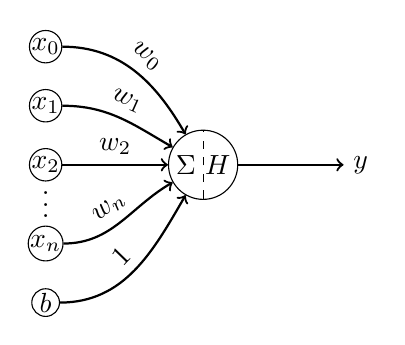
\begin{tikzpicture}
\node[draw,circle,minimum size=25pt,inner sep=0pt] (x) at (0,0) {$\Sigma$ $H$};
\node[] (y) at (2,0) {$y$};

\node[inputNode] (x0) at (-2, 1.5) {$x_0$};
\node[inputNode] (x1) at (-2, 0.75) {$x_1$};
\node[inputNode] (x2) at (-2, 0) {$x_2$};
\node[inputNode] (xn) at (-2, -1.0) {$x_n$};
\node[inputNode] (b) at (-2, -1.75) {$b$};

\draw[stateTransition] (x0) to[out=0,in=120] node [midway, sloped, above] {$w_0$} (x);
\draw[stateTransition] (x1) to[out=0,in=150] node [midway, sloped, above] {$w_1$} (x);
\draw[stateTransition] (x2) to[out=0,in=180] node [midway, sloped, above] {$w_2$} (x);
\draw[stateTransition] (xn) to[out=0,in=210] node [midway, sloped, above] {$w_n$} (x);
\draw[stateTransition] (b) to[out=0,in=240] node [midway, sloped, above] {$1$}(x);
\draw[stateTransition] (x) to node [midway,above=-0.1cm] {}(y);
\draw[dashed] (0,-0.43) -- (0,0.43);
\node (dots) at (-2, -0.4) {$\vdots$};
\end{tikzpicture}
	\caption{Aufbau eines Neurons äquivalent zur Gleichung \ref{eq:neuron}.}
	\label{fig:neuron}
\end{figure}

\subsection{Convolutional Neural Nets}

Eine Unterkategorie der KNNs stellen die Convolutional Neural Nets (CNN) dar.
Wie der Name schon sagt, spielen dabei Faltungen eine wichtige Rolle.
Bevor die normalen KNN Layer kommen, werden Bilddaten üblicherweise zuerst von einigen Faltungslayern vorverarbeitet.
Die Idee dazu kommt von der klassischen Bildverarbeitung, wo häufig Faltungskernel verwendet werden um ein Bild zu filtern oder Features zu erkennen.
Bei einem CNN werden diese Kernel nicht vom Ingenieur bestimmt, sondern während Trainings durch den Algorithmus gelernt.  
Die gelernten Gewichte (Kernels) haben an jeder Position der Faltung die selben Werte, sind also Translationsinvariant.
Diese Eigenschaft ist entscheidend, da sie einerseits die Anzahl zu lernender Gewichte extrem reduziert und andererseits die Generalisierung fördert.
Solche CNNs zeigen extrem gute Resultate in der Bildverarbeitung, speziell im Bereich der Klassifizierung von Bildern (z.B. Erkennen von Katzen).
Wie eine zweidimensionale Faltung funktioniert ist in Abbildung \ref{fig:2dconv} gezeigt.

\begin{figure}
	\centering
	\usetikzlibrary{matrix, positioning}
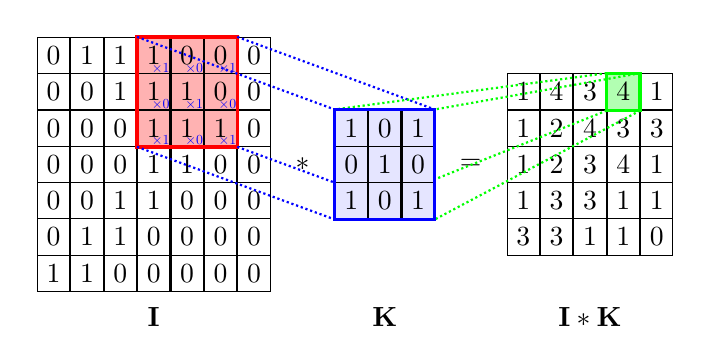
\begin{tikzpicture}

	\matrix (mtr) [matrix of nodes,row sep=-\pgflinewidth, nodes={draw}]
	{
		0 & 1 & 1 & |[fill=red!30]| 1 & |[fill=red!30]| 0 & |[fill=red!30]| 0 & 0\\
		0 & 0 & 1 & |[fill=red!30]| 1 & |[fill=red!30]| 1 & |[fill=red!30]| 0 & 0\\
		0 & 0 & 0 & |[fill=red!30]| 1 & |[fill=red!30]| 1 & |[fill=red!30]| 1 & 0\\
		0 & 0 & 0 & 1 & 1 & 0 & 0\\
		0 & 0 & 1 & 1 & 0 & 0 & 0\\
		0 & 1 & 1 & 0 & 0 & 0 & 0\\
		1 & 1 & 0 & 0 & 0 & 0 & 0\\
	};

	\draw[very thick, red] (mtr-1-4.north west) rectangle (mtr-3-6.south east);

	\node [below= of mtr-5-4.south] (lm) {$\bf I$};

	\node[right = 0.2em of mtr] (str) {$*$};

	\matrix (K) [right=0.2em of str,matrix of nodes,row sep=-\pgflinewidth, nodes={draw, fill=blue!30}]
	{
		1 & 0 & 1 \\
		0 & 1 & 0 \\
		1 & 0 & 1 \\
	};
	\node [below = of K-3-2.south] (lk) {$\bf K$};

	\node [right = 0.2em of K] (eq) {$=$};

	\matrix (ret) [right=0.2em of eq,matrix of nodes,row sep=-\pgflinewidth, nodes={draw}]
	{
		1 & 4 & 3 & |[fill=green!30]| 4 & 1\\
		1 & 2 & 4 & 3 & 3\\
		1 & 2 & 3 & 4 & 1\\
		1 & 3 & 3 & 1 & 1\\
		3 & 3 & 1 & 1 & 0\\
	};
	\node [below = of ret-4-3.south] (lim) {${\bf I} * {\bf K}$};

	\draw[very thick, green] (ret-1-4.north west) rectangle (ret-1-4.south east);

	\draw[densely dotted, blue, thick] (mtr-1-4.north west) -- (K-1-1.north west);
	\draw[densely dotted, blue, thick] (mtr-3-4.south west) -- (K-3-1.south west);
	\draw[densely dotted, blue, thick] (mtr-1-6.north east) -- (K-1-3.north east);
	\draw[densely dotted, blue, thick] (mtr-3-6.south east) -- (K-3-3.south east);

	\draw[densely dotted, green, thick] (ret-1-4.north west) -- (K-1-1.north west);
	\draw[densely dotted, green, thick] (ret-1-4.south west) -- (K-3-1.south west);
	\draw[densely dotted, green, thick] (ret-1-4.north east) -- (K-1-3.north east);
	\draw[densely dotted, green, thick] (ret-1-4.south east) -- (K-3-3.south east);

	\matrix (K) [right=0.2em of str,matrix of nodes,row sep=-\pgflinewidth, nodes={draw, fill=blue!10}]
	{
		1 & 0 & 1 \\
		0 & 1 & 0 \\
		1 & 0 & 1 \\
	};

	\draw[very thick, blue] (K-1-1.north west) rectangle (K-3-3.south east);

	\node[anchor=south east, inner sep=0.01em, blue] at (mtr-1-4.south east) (xx) {\scalebox{.5}{$\times 1$}};
	\node[anchor=south east, inner sep=0.01em, blue] at (mtr-1-5.south east) (xx) {\scalebox{.5}{$\times 0$}};
	\node[anchor=south east, inner sep=0.01em, blue] at (mtr-1-6.south east) (xx) {\scalebox{.5}{$\times 1$}};
	\node[anchor=south east, inner sep=0.01em, blue] at (mtr-2-4.south east) (xx) {\scalebox{.5}{$\times 0$}};
	\node[anchor=south east, inner sep=0.01em, blue] at (mtr-2-5.south east) (xx) {\scalebox{.5}{$\times 1$}};
	\node[anchor=south east, inner sep=0.01em, blue] at (mtr-2-6.south east) (xx) {\scalebox{.5}{$\times 0$}};
	\node[anchor=south east, inner sep=0.01em, blue] at (mtr-3-4.south east) (xx) {\scalebox{.5}{$\times 1$}};
	\node[anchor=south east, inner sep=0.01em, blue] at (mtr-3-5.south east) (xx) {\scalebox{.5}{$\times 0$}};
	\node[anchor=south east, inner sep=0.01em, blue] at (mtr-3-6.south east) (xx) {\scalebox{.5}{$\times 1$}};

\end{tikzpicture}
	\caption{Darstellung einer zweidimensionalen Faltung des Bildes $I$ mit dem Kernel $K$.}
	\label{fig:2dconv}
\end{figure}

Anhand von der Bildverarbeitung kann man den Unterschied von KNNs und CNNs gut erklären.
Bei einem KNN wird jedes Pixel mit jedem Neuron verbunden und für jede dieser Verbindungen wird ein eigenes Gewicht gelernt.
Beim CNN hingegen wird ein einzelner Kernel gelernt, welcher dann translationsinvariant auf das ganze Bild angewendet wird.
Als Beispiel nehmen wir einen ersten Layer von $256$ Neuronen, ein Eingangsbild der Grösse $128\times128$ und eine Kernelgrösse von $3\times3$.
Damit erhalten wir beim KNN	$256 \cdot 128 \cdot 128 = 4'227'072$ Gewichte welche gelernt werden müssen.
Beim CNN hingegen genügen $256 \cdot 3 \cdot 3 = 2'304$ Gewichte.

Die zweidimensionale Wavelet-Transformation kann auch als Faltung des Bildes mit dem Wavelet (Kernel) interpretiert werden.
Dabei werden allerdings nicht mehr alle kontinuierlichen Grössen des Wavelets berücksichtigt, sondern nur noch eine diskrete Anzahl.
Da KNNs (und CNNs) vom Hirn inspirierte Algorithmen darstellen und die Bildvorverarbeitung im Hirn als Gabor-Wavelet-Transformation modelliert werden kann, drängt sich daher eine Kombination dieser beiden Konzepte auf.

Eine offensichtliche Idee ist dabei das Vorverabeiten der Bilder mithilfe von Gabor-Wavelets.
Diese vorverarbeiteten Bilder können dann als Input in das CNN verwendet werden und sollten gute Resultate zeigen, analog zum menschlichen Hirn.
Ob diese theoretischen Ideen auch praktisch anwendbar sind, soll ein Versuch zeigen.

\subsection{Versuch}

Das Ziel des Versuches ist es, zu zeigen ob Gabor-Wavelets wirklich eine Berechtigung im Zusammenhang mit CNNs haben.
Zwei verschiedene Dinge sollen überprüft werden:
\begin{enumerate}
	\item Ist eine vorverarbeitung mittels Gabor-Kerneln sinnvoll?
	\item Lernt ein CNN Kernels welche Ähnlichkeiten zu den Gabor-Kerneln besitzen?
\end{enumerate}
Um diese Ziele zu erreichen wurde ein Versuch durchgeführt, bei welchem der CIFAR-10 \cite{paper:cifar10} Datensatz klassifiziert werden soll.
Beim CIFAR-10 Datensatz handelt es sich um $32 \times 32$ Pixel grosse farbige Bilder,welche zu zehn verschiedenen Klassen gehören (z.B. Flugzeug, Vogel, etc.).
Der Datensatz umfasst dabei 50'000 Trainings- und 10'000 Testbilder.
Ein Beispiel jeder Klasse ist in Abbildung \ref{fig:cifar10} gezeigt.
Der CIFAR-10 Datensatz wurde gewählt da er ziemlich bekannt ist, Beispielarchitekturen verfügbar sind und relativ schwierig zu lösen ist.
Die Schwierigkeit ist wichtig um überhaupt einen Unterschied in der Genauigkeit feststellen zu können (bei 99\% Genauigkeit sieht man keine grossen Verbesserungen mehr).

\begin{figure}
	\centering
	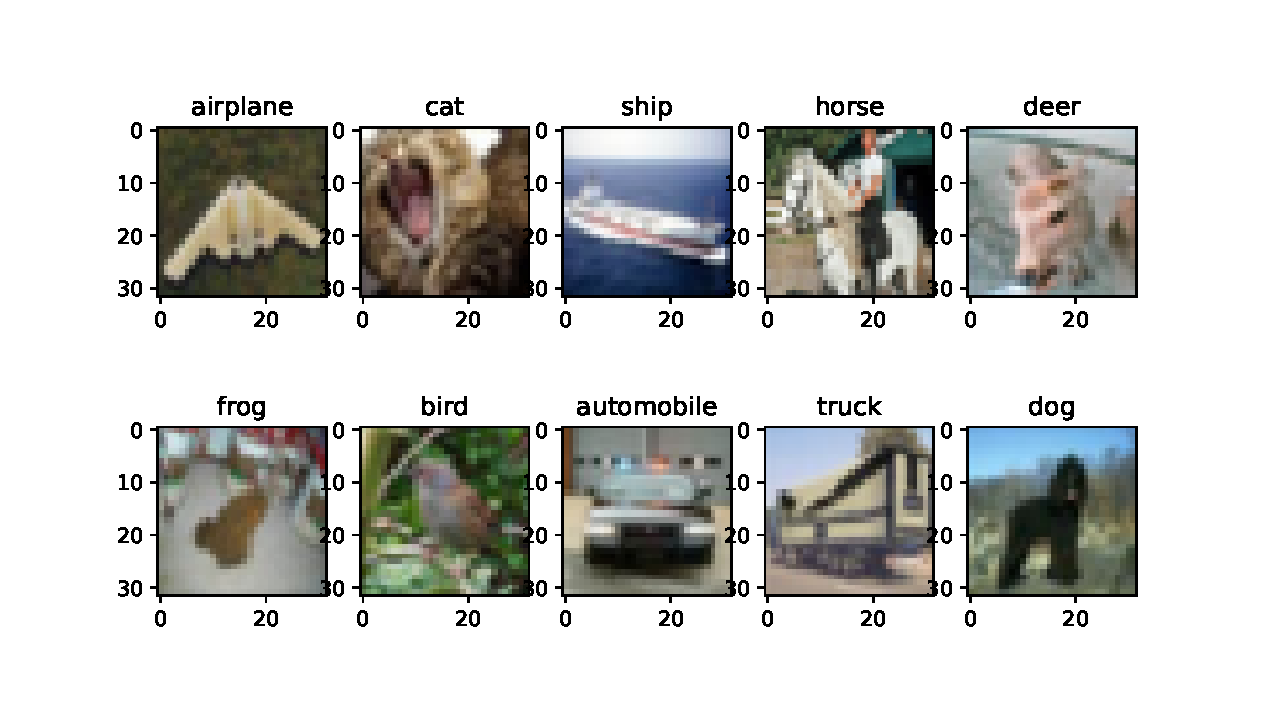
\includegraphics[width=0.6\linewidth, trim=0 60 0 40, clip]{./papers/visuell/images/cifar10}
	\caption{Die zehn verschiedenen Klassen des CIFAR-10 Datensatzes.}
	\label{fig:cifar10}
\end{figure}

Die Architektur des CNNs ist inspiriert von einem Artikel über CIFAR-10 \cite{online:cifar10}.
Implementiert wurde das gesamte Projekt mit Python und Tensorflow.

Der erste Convolutional-Layer besteht aus $64$ verschiedenen $9 \times 9$ Kerneln, welche entweder gelernt werden oder als Gabor-Kernels gesetzt werden.
Also wird das Netzwerk zwei mal trainiert, einmal mit einem fixen ersten Layer (Gabor-Layer) und einmal mit einem lernbaren ersten Layer.
Die Variante mit Gabor-Layer stellt dem Netzwerk weniger Freiheitsgrade zur Verfügung und sollte theoretisch ein schlechteres Resultat zeigen.
Da wir aber vermuten das ein Gabor-Layer eine optimale Vorverarbeitung darstellt, sollten die Gabor-Kernels besser Resultate als die selbst gelernten zeigen.

Nach dem ersten Layer folgen drei weitere Convolutional-Layer, bevor am Ende fünf Fully-Connected-Layer (normale KNN-Layer) das Resultat ausgeben.
Die genaue Architektur ist in Tabelle \ref{table:architecture} gezeigt.
Die Bilder werden zuerst in schwarzweiss Bilder umgewandelt, damit die Gabor-Variante keinen Nachteil bekommt.
Der Nachteil würde entstehen, da das Netzwerk für jede Farbe andere Features lernen könnte, wohingegen die Gabor-Variante auf allen Farben die gleichen Kernels benutzen würde. 

\begin{table}
	\centering
	\begin{tabular}{|c|c|c|}
		\hline
		Layer & Kernelgrösse & Ausgangsgrösse \\ 
		\hline \hline
		Input & - & $32 \times 32 \times 1$ \\ 
		\hline 
		Conv1 & $9 \times 9$ &  $32 \times 32 \times 64$\\ 
		\hline 
		Conv2 & $3 \times 3$ &  $32 \times 32 \times 128$\\  
		\hline 
		Pool2 & - &  $16 \times 16 \times 128$\\ 
		\hline 
		Conv3 & $3 \times 3$ & $16 \times 16 \times 256$\\ 
		\hline 
		Pool3 & - &  $8 \times 8 \times 256$\\ 
		\hline 
		Conv4 & $3 \times 3$ & $8 \times 8 \times 512$\\ 
		\hline 
		Pool4 & - &  $4 \times 4 \times 512$\\ 
		\hline 
		Flatten & - & $ 8192 $ \\ 
		\hline 
		FC1 & - & $ 128 $ \\ 
		\hline 
		FC2 & - & $ 256 $ \\
		\hline 
		FC3 & - & $ 512 $ \\  
		\hline 
		FC4 & - & $ 1024 $ \\ 
		\hline 
		Softmax & - & $ 10 $ \\ 
		\hline
	\end{tabular} 
	\caption{Unsere Netzwerk-Architektur. Der erste Layer (Conv1) wird bei der Gabor-Variante fix gesetzt und nicht gelernt. Nach jedem Convolutional- und Fully-Connected-Layer wird eine Batch-Normalization durchgeführt. Die Aktivierungsfunktion ist immer ReLu, ausser beim Softmax-Output.}
	\label{table:architecture}
\end{table}



\section{Resultate}
\rhead{Resultate}

Die Ergebnisse des Versuches sind erstaunlich eindeutig.
Die Variante mit Gabor-Kerneln erreicht immer höhere Genauigkeiten als die klassische CNN Variante.
Gleichzeitig müssen bei der Gabor Variante weniger Gewichte gelernt werden, weshalb die Trainingszeit reduziert wird.
Also werden nicht nur bessere Resultate erreicht, es werden auch noch weniger Ressourcen für das Training benötigt.

In Abbildung \ref{fig:acc} sind die Genauigkeiten der beiden Varianten über fünf Trainingsepochen gezeigt.
Eine Epoche entspricht dabei einem kompletten Trainingsdurchgang durch den gesamten Trainingsdatensatz.
Beide Varianten sind 10 mal trainiert worden. 
Es zeigt sich, dass die Variante mit dem fixen Gabor-Layer in allen 10 Fällen eine höhere Genauigkeit aufweist.
Die kleinste Genauigkeit der Gabor-Variante nach 5 Epochen beträgt 67.32\% und die höchste Genauigkeit der klassischen Variante 66.42\%.
Somit haben wir eine Lücke zwischen den beiden Varianten von ca. 1\%.
Falls über eine längere Zeit trainiert wird (z.B. 20 Epochen), verändern sich die Resultate nur minimal und der Unterschied der beiden Varianten bleibt bestehen.
Unsere Resultate bestätigen also die Hypothese \ref{hyp:1}.

\begin{figure}
	\centering
	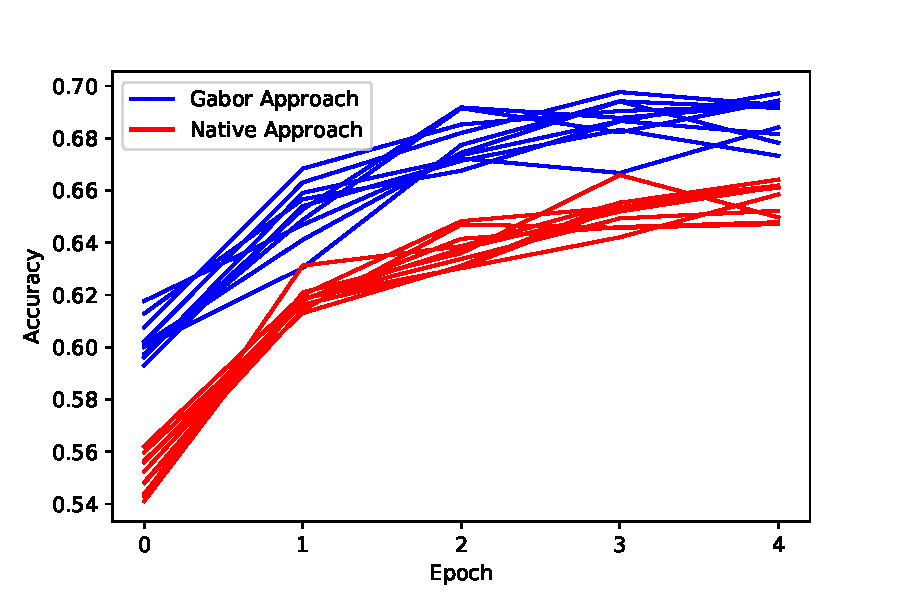
\includegraphics[width=0.7\linewidth]{./papers/visuell/images/accuracy}
	\caption{Test-Genauigkeit (Accuracy) der beiden Varianten im Laufe des Trainings.}
	\label{fig:acc}
\end{figure}

Entscheidend bei neuronalen Netzen sind neben der Genauigkeit die Geschwindigkeiten für das Trainieren und Klassifizieren.
Bei der Variante mit Gabor dauerte das Training etwa 3 Minuten und 10 Sekunden (kann abhängig vom Computer und Grafikkarte stark variieren).
Bei der zweiten Variante, wo erste Layer ebenfalls gelernt wird, dauert das Training ca. 15\% länger (also etwa 3 Minuten und 38 Sekunden).
Das Klassifizieren von neuen Bildern dauert danach bei beiden Varianten gleich lange, da in beiden Fällen die identische Tensorflow-Struktur implementiert wurde.

Lernt das klassische CNN Kernels welche Ähnlichkeiten zu Gabor-Wavelets aufweisen?
In unserem Versuch ist dies nicht der Fall.
Die Kernel welche gelernt wurden sehen zufällig aus, es sind keine Regelmässigkeiten zu erkennen.
Abbildung \ref{fig:cnnkernels} zeigt diese gelernten Kernels, welche mit den Gabor-Kernels in Abbildung \ref{fig:cnngkernels} verglichen werden sollten.
Durch die zufällige Initialisierung ist es aber nicht ausgeschlossen, dass solche Gabor-Ähnlichen Kernels gelernt werden könnten.
Es gibt Beispiele von CNN-Kernels, welche Ähnlichkeiten zu Gabor-Kernels aufweisen (vgl. Kapitel 9.10 im Buch \cite{book:deeplearning}).
Die Vermutung liegt nahe, dass durch die kleine Auflösung der CIFAR-10 Bilder solch komplexe Kernels nicht gelernt wurden.

\begin{figure}
	\centering
	\subfigure{
\includegraphics[width=0.3\linewidth]{./papers/visuell/images/kernel1}}
	\subfigure{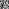
\includegraphics[width=0.3\linewidth]{./papers/visuell/images/kernel2}}
	\subfigure{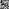
\includegraphics[width=0.3\linewidth]{./papers/visuell/images/kernel3}}
	\caption{Drei verschiedene Kernels des ersten Layers welche vom Netzwerk gelernt wurden. Es sind keine Regelmässigkeiten erkennbar.}
	\label{fig:cnnkernels}
\end{figure}

\begin{figure}
	\centering
	\subfigure{
\includegraphics[width=0.3\linewidth]{./papers/visuell/images/kernelG1}}
	\subfigure{
\includegraphics[width=0.3\linewidth]{./papers/visuell/images/kernelG2}}
	\subfigure{
\includegraphics[width=0.3\linewidth]{./papers/visuell/images/kernelG3}}
	\caption{Drei verschiedene Gabor-Kernels des ersten Layers.}
	\label{fig:cnngkernels}
\end{figure}


\section{Schlussfolgerung}
\rhead{Schlussfolgerung}



\printbibliography[heading=subbibliography]
\end{refsection}
